%%%%%%%%%%%%%%%%%%%%%%%%%%%%%%%%%%%%
%                                  %
% Titre  : m_f.tex                 %
% Sujet  : Maintenance manual of   %
%          Scotch                  %
%          File formats v6.0       %
% Auteur : Francois Pellegrini     %
%                                  %
%%%%%%%%%%%%%%%%%%%%%%%%%%%%%%%%%%%%

\section{Files and data structures}
\label{sec-file}

User-manageable file formats are described in the \scotch user's
guide. This section contains information that are relevant only to
developers and maintainers.

For the sake of portability, readability, and reduction of storage space,
all the data files shared by the different programs of the
\scotch\ project are coded in plain ASCII text exclusively.
Although one may speak of ``lines'' when describing file formats,
text-formatting characters such as newlines or tabulations are not
mandatory, and are not taken into account when files are read.
They are only used to provide better readability and understanding.
Whenever numbers are used to label objects, and unless explicitely
stated, \textbf{numberings always start from zero}, not one.

\subsection{Decomposition-defined architecture files}
\label{sec-file-target-deco-one}

Decomposition-defined architecture files are the way to describe
irregular target architectures that cannot be represented as
algorithmically-coded architectures.

Two main file formats coexist: the ``\texttt{deco 0}'' and
``\texttt{deco 2}'' formats. ``\texttt{deco}'' stands for
``decomposition-defined architecture'', followed by the format
number. The ``\texttt{deco 1}'' format is a compiled form of the
``\texttt{deco 0}'' format. We will describe it here.

The ``\texttt{deco 1}'' file format results from an $O(p^2)$
preprocessing of the ``\texttt{deco 0}'' target architecture
format. While the ``\texttt{deco 0}'' format contains a distance
matrix between all pairs of terminal domains, which is consequently in
in $\Theta(p^2/2)$, the ``\texttt{deco 1}'' format contains the
distance matrix between any pair of domains, whether they are terminal
or not. Since there are roughly $2p$ non-terminal domains in a
target architecture with $p$ terminal domains, because all domains
form a binary tree whose leaves are the terminal domains, the distance
matrix of a ``\texttt{deco 1}'' format is in $\Theta(2p^2)$, that is,
four times that of the corresponding ``\texttt{deco 0}'' file.

Also, while the ``\texttt{deco 0}'' format lists only the
characteristics of terminal domains (in terms of weights and labels),
the ``\texttt{deco 1}'' format provides these for all domains, so as
to speed-up the retrieval of the size, weight and label of any domain,
whether it is terminal or not.

The ``\texttt{deco 1}'' header is followed by two integer numbers,
which are the number of processors and the largest terminal number used
in the decomposition, respectively (just as for ``\texttt{deco 0}''
files). Two arrays follow.

The first array has as many lines as there are domains (and not only
terminal domains as in the case of ``\texttt{deco 0}'' files). Each of
these lines holds three numbers: the label of the terminal domain that
is associated with this domain (which is the label of the terminal
domain of smallest number contained in this domain), the size of the
domain, and the weight of the domain.
The first domain in the array is the initial domain holding all the
processors, that is, domain $1$. The other domains in the array are
the resulting subdomains, in ascending domain number order, such that
the two subdomains of a given domain of number $i$ are numbered $2i$
and $2i+1$.

The second array is a lower triangular diagonal-less matrix that gives the
distance between all pairs of domains.

For instance, Figure~\ref{fig-file-targetdeco-zero} and
Figure~\ref{fig-file-targetdeco-one} show the contents of the
``\texttt{deco 0}'' and ``\texttt{deco 1}'' architecture decomposition
files for $\UB(2,3)$, the binary de~Bruijn graph of dimension~$3$, as
computed by the \texttt{amk\_grf} program.
\begin{figure}[hbt]
\begin{tabular}{p{0.69\linewidth}@{}p{0.29\linewidth}}
\begin{center}
\parbox[t]{0.9\linewidth}{\vspace{0pt}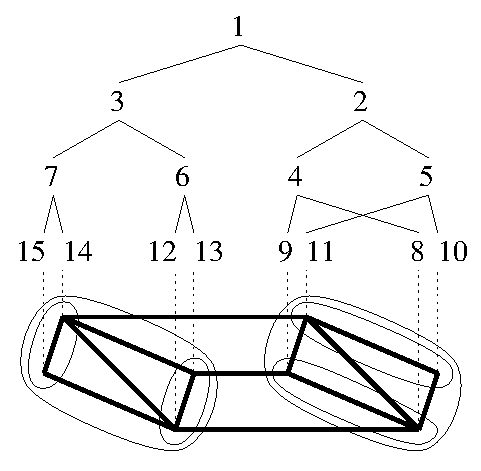
\includegraphics[width=0.7\linewidth]{s_f_d.ps}}
\end{center}
&
\begin{center}
{\renewcommand{\baselinestretch}{1.05}
\footnotesize\tt
\begin{verbatim}
deco 0
8	15
0	1	15
1	1	14
2	1	13
3	1	11
4	1	12
5	1	9
6	1	8
7	1	10
1
2 1
2 1 2
1 1 1 2
3 2 1 1 2
2 2 2 1 1 1
3 2 3 1 2 2 1
\end{verbatim}
}
\end{center}
\end{tabular}
\caption{``\texttt{deco 0}'' target decomposition file for $\UB(2,3)$.
         The terminal numbers associated with every processor define a unique
         recursive bipartitioning of the target graph.}
\label{fig-file-targetdeco-zero}
\end{figure}

\begin{figure}[hbt]
\begin{tabular}{p{0.49\linewidth}@{}p{0.49\linewidth}}
\begin{center}
{\renewcommand{\baselinestretch}{1.05}
\footnotesize\tt
\begin{verbatim}
deco
1
8	15
0	8	8
3	4	4
0	4	4
5	2	2
3	2	2
2	2	2
0	2	2
6	1	1
5	1	1
7	1	1
3	1	1
4	1	1
2	1	1
1	1	1
0	1	1
\end{verbatim}
}
\end{center}
&
\begin{center}
{\renewcommand{\baselinestretch}{1.05}
\footnotesize\tt
\begin{verbatim}
2	2	2	2	1	2	2	1
3	1	2	2	1	2	2	2
3	1	2	2	1	2	1	2
1	1	2	2	3	2	3	1
2	2	3	1	3	2	3	2
1	3	3	1	2	2	1	2
1	1	2	2	1	1	1	2
2	1	2	2	1	1	1	2
2	2	3	3	2	2	3	1
2	2	1	3	2	1	2	2
1	2	2	1	1	2	2	2
1	1	1	3	3	2	3	3
2	1	2	3	3	2	1	2
1
\end{verbatim}
}
\end{center}
\end{tabular}
\caption{``\texttt{deco 1}'' target decomposition file for $\UB(2,3)$,
  compiled with the \texttt{acpl} tool from the ``\texttt{deco 0}''
  file displayed in Figure~\ref{fig-file-targetdeco-zero}.}
\label{fig-file-targetdeco-one}
\end{figure}
